\documentclass[10pt,letterpaper]{article}

% -----------------------------------------------------------------------------
% Measuring What We Mean — position paper v6
% Fusion: v5 general-science spine + v4 formal payload + first-principles SI
% Empty empirical results (deferred to cvprofiles v3); synthetic DGPs only
% -----------------------------------------------------------------------------
\usepackage[margin=0.88in,top=0.82in,bottom=0.82in]{geometry}
\usepackage{mathptmx}
\usepackage[T1]{fontenc}
\usepackage{microtype}
\usepackage{amsmath,amssymb}
\usepackage{amsthm}
\newtheorem{proposition}{Proposition}[section]
\newtheorem{definition}{Definition}[section]
\newtheorem{remark}{Remark}[section]
\newtheorem{assumption}{Assumption}[section]
\usepackage{booktabs,array,tabularx}
\usepackage{ifthen}
\usepackage{graphicx}
\usepackage{tikz}
\usetikzlibrary{arrows.meta,positioning,shapes.geometric,calc,fit,backgrounds}
\usepackage{xcolor}
\usepackage{hyperref}
\usepackage{enumitem}
\usepackage{titlesec}
\usepackage{caption}
\usepackage{fancyhdr}
\usepackage{multirow}

\definecolor{econblue}{RGB}{20,55,95}
\definecolor{slate}{RGB}{79,89,104}
\definecolor{mist}{RGB}{242,245,249}
\definecolor{rulegray}{RGB}{203,210,220}
\definecolor{warm}{RGB}{132,85,38}
\definecolor{passgreen}{RGB}{42,104,78}
\definecolor{failred}{RGB}{150,55,55}
\definecolor{amber}{RGB}{170,120,40}

\hypersetup{colorlinks=true,linkcolor=econblue,citecolor=econblue,urlcolor=econblue,
  pdftitle={Measuring What We Mean: Construct Validity When Measures Are Cheap},
  pdfauthor={Augusto Gonzalez-Bonorino, Kseniia Biriukova, and Monica Capra}}
\setlength{\parindent}{1.15em}
\setlength{\parskip}{0.18em}
\setlength{\headheight}{20pt}
\titlespacing*{\section}{0pt}{1.0em}{0.3em}
\titlespacing*{\subsection}{0pt}{0.68em}{0.22em}
\titleformat{\section}{\large\bfseries\color{econblue}}{\thesection.}{0.55em}{}
\titleformat{\subsection}{\normalsize\bfseries\color{econblue}}{\thesubsection}{0.45em}{}
\setlist[itemize]{leftmargin=1.3em,itemsep=0.12em,topsep=0.15em}
\setlist[enumerate]{leftmargin=1.45em,itemsep=0.12em,topsep=0.15em}
\captionsetup{font=small,labelfont={bf,color=econblue},skip=4pt}

\pagestyle{fancy}
\fancyhf{}
\fancyhead[L]{\small\color{slate} EconLLM Lab \textperiodcentered\ Position paper v6}
\fancyhead[R]{\small\color{slate}\thepage}
\renewcommand{\headrulewidth}{0.35pt}
\renewcommand{\headrule}{\hbox to\headwidth{\color{rulegray}\leaders\hrule height \headrulewidth\hfill}}
\fancypagestyle{plain}{\fancyhf{}\fancyfoot[C]{\small\color{slate}\thepage}\renewcommand{\headrulewidth}{0pt}}

\newcommand{\SCA}{\textsc{sca}}
\newcommand{\LLM}{\textsc{llm}}
\newcommand{\DPO}{\textsc{dpo}}
\newcommand{\GPS}{\textsc{gps}}
\newcommand{\WVS}{\textsc{wvs}}
\newcommand{\WEIRD}{\textsc{weird}}
\newcommand{\cvp}{\texttt{cvprofiles}}
\newcommand{\M}{\ensuremath{\mathcal{M}}}
\newcommand{\E}{\mathbb{E}}
\newcommand{\Rset}{\mathcal{R}}
\newcommand{\Bset}{\mathcal{B}}

\begin{document}

% =============================================================================
% Cover
% =============================================================================
\thispagestyle{empty}
\begin{center}
\vspace*{1.1cm}
{\color{econblue}\rule{\textwidth}{1.15pt}}\\[0.45em]
{\LARGE\bfseries\color{econblue} Measuring What We Mean}\\[0.16em]
{\LARGE\bfseries\color{econblue} Construct Validity When Measures Are Cheap}\\[0.45em]
{\color{econblue}\rule{\textwidth}{0.55pt}}\\[0.75em]
{\large A position paper on measurement selection in the age of AI}\\[0.95em]
{\large\textbf{Augusto Gonzalez-Bonorino}\textsuperscript{1}\quad
\textbf{Kseniia Biriukova}\textsuperscript{2}\quad
\textbf{Monica Capra}\textsuperscript{1,3}}\\[0.5em]
{\small\textsuperscript{1}Department of Economics, Arizona State University; EconLLM Lab.\\
\textsuperscript{2}EconLLM Lab.\\
\textsuperscript{3}Department of Economics, Claremont Graduate University; EconLLM Lab.}\\[0.75em]
{\normalsize August 2026 \textperiodcentered\ Working paper / position paper}\\[0.35em]
{\color{econblue}\rule{0.28\textwidth}{0.35pt}}
\end{center}

\vspace{0.6em}
\noindent\colorbox{mist}{\parbox{0.965\textwidth}{\small\vspace{0.3em}
\textbf{Status.} This document states a research program and the evidence required to support it.
Empirical results on real survey and AI measures are \emph{intentionally empty}: they are blocked until the companion validation engine \cvp{} ships the v3 inference and holdout layers needed for the intended analysis.
What follows is the framework, its first-principles derivation, controlled synthetic illustrations of the shipped v2 engine, and a preregistered plan for the real-world proof of concept.
Code: \href{https://github.com/EconLLM-Lab/SCA2_PofW}{\texttt{SCA2\_PofW}}; engine: \href{https://github.com/Bonorinoa/cvprofiles}{\texttt{cvprofiles}}.
\vspace{0.3em}}}

\vspace{0.85em}
\section*{Statement of significance}
Scientists rarely observe constructs such as trust, ideology, culture, or risk preference directly. They work through measures.
Artificial intelligence changes the economics of this problem: researchers can now generate many plausible measures quickly---prompted responses, embeddings, classifiers, synthetic agents, fine-tuned policies.
When measures become cheap, choosing and validating them becomes the scarce scientific task.

This paper proposes a simple discipline.
Define the construct; declare a menu of candidate measures; state observable validity tests implied by the construct; retain the measures that survive; and report which scientific conclusions are robust across the surviving set.
The framework treats conventional survey measures and AI-generated measures symmetrically.
It completes, operationally, a construct-validity program that recent econometric work formalized as partial identification over measurement menus and left open at the inference stage~\cite{dellrambachan2026}.
The intended contribution is not a new definition of construct validity, but a general, auditable way to use construct-validity evidence to select among heterogeneous measures and propagate remaining measurement uncertainty into scientific conclusions---implemented in open software, illustrated on controlled data-generating processes, and designed for a real-world cultural-preferences application once the technology supports the required analysis.

\section*{Abstract}
Artificial intelligence has sharply reduced the cost of producing candidate measures of latent constructs.
A researcher can measure trust, sentiment, ideology, or cultural preference with a survey item, a composite score, a prompted language model, or a fine-tuned policy.
The resulting abundance creates a selection problem: which measures warrant the interpretation researchers give them, and which empirical conclusions survive reasonable measurement choice?
Measurement selection is formulated around four objects: a construct $C$, a declared menu of candidate measures $\M$, a set of theory-derived validity tests $\Rset$, and a scientific result $\theta(m)$ computed using measure $m$.
The tests define a surviving set $\M^*$; the image $\Theta^*=\{\theta(m):m\in\M^*\}$ reports the conclusions robust to measurement choice within the declared menu and validity argument.
Held-out validity tests make the selection rule itself falsifiable.
The framework is derived from first principles as partial identification over a finite menu of measurement functions, with maintained assumptions, a consistency proposition for the plug-in admissible set and range, and a mandatory additive reporting layer for sampling uncertainty induced by data-dependent screening.
It is implemented in the open, model-free package \cvp{}.
Controlled synthetic data-generating processes illustrate the shipped engine and the limitations that motivate the next release.
Empirical results on real survey and AI measures are deferred until that release; a preregistered trust-and-preferences study is specified as the real-world proof of concept.
The broader research agenda is to make measurement selection auditable when candidate measures are abundant.

\noindent\textbf{Keywords:}
measurement selection; construct validity; partial identification; AI measurement; synthetic cultural agents; cultural preferences; trust

% =============================================================================
\section{When measures become cheap}
% =============================================================================
Empirical science often begins with a concept that is scientifically meaningful but not directly observed.
Trust, patience, reciprocity, ideology, polarization, and culture are familiar examples.
Let $C$ denote such a construct.
Researchers learn about $C$ through an operationalization $m$: a survey question, scale, experimental task, administrative proxy, factor score, text classifier, or other procedure that produces an observable score or response.
The measure is not the construct.
Its scientific value depends on whether the interpretation attached to its output is warranted.

For much of social science, producing a new measure was costly.
Artificial intelligence relaxes this constraint.
Large language models can label text, answer surveys, simulate respondents, generate scales, produce embeddings, and be adapted to represent target populations at low marginal cost~\cite{horton2023,argyle2023,aher2023,manning2024,gilardi2023}.
The change in cost does not remove the measurement problem; it changes its location.
If a prompt, embedding, composite, or fine-tuned model can be generated quickly, the scarce resource is no longer a candidate operationalization---it is evidence that the operationalization measures what the researcher means.

Recent audits of \LLM{} use in social science find that model-generated measurements increasingly enter substantive analyses while validation practices remain heterogeneous~\cite{desai2026}.
At the 2026 Political Methodology meetings, generative AI was central in roughly a quarter of presentations, and most of that work was measurement-related~\cite{hall2026}.
Computational social science and NLP have begun importing construct-validity language explicitly~\cite{proxy2026,halterman2024,bean2025}.
Our premise is that this trend should be generalized beyond any one AI method: when measures are cheap, validity becomes the scarce resource.

That premise has a precise econometric home.
Dell and Rambachan's 2026 NBER Methods Lectures formalize the Cronbach--Meehl nomological network as a partial-identification problem over a menu of candidate measures, with moment-inequality restrictions, an admissible set, and a construct-identified range for a downstream estimand---and they explicitly leave estimation and inference beyond the lecture's scope~\cite{dellrambachan2026,cronbach1955}.
This paper completes that program end-to-end: the decision rule, the inference protocol for data-dependent screening, the open implementation, and a planned cultural application.
The contribution is operational and auditable, not a claim to have discovered the bridge.

\begin{figure}[t]
\centering
\begin{tikzpicture}[
  font=\small,
  box/.style={draw=econblue, rounded corners=3pt, fill=mist, align=center,
              text width=2.35cm, minimum height=1.15cm, inner sep=5pt, line width=0.7pt},
  arr/.style={-{Stealth[length=2.2mm]}, line width=0.9pt, color=slate}]
\node[box] (C) {\textbf{Construct $C$}\\[2pt]{\scriptsize\color{slate}What do we mean?}};
\node[box, right=0.55cm of C] (M) {\textbf{Menu $\M$}\\[2pt]{\scriptsize\color{slate}How might we measure it?}};
\node[box, right=0.55cm of M] (R) {\textbf{Tests $\Rset$}\\[2pt]{\scriptsize\color{slate}What should a valid measure do?}};
\node[box, right=0.55cm of R] (Ms) {\textbf{Survivors $\M^*$}\\[2pt]{\scriptsize\color{slate}Which measures pass?}};
\node[box, below=0.85cm of Ms, fill=passgreen!12, draw=passgreen] (Th)
  {\textbf{Robust set $\Theta^*$}\\[2pt]{\scriptsize\color{slate}Which conclusions survive?}};
\draw[arr] (C)--(M); \draw[arr] (M)--(R); \draw[arr] (R)--(Ms);
\draw[arr] (Ms)--(Th);
\node[font=\scriptsize\color{slate}, left=0.15cm of Th, align=right, text width=4.2cm]
  {Propagate measurement choice\\into the scientific result $\theta(m)$};
\end{tikzpicture}
\caption{Core objects of the framework.
The same five terms appear in prose, figures, and formal statements throughout.}
\label{fig:core}
\end{figure}

% =============================================================================
\section{One construct, many measures}
% =============================================================================
The paper uses a deliberately small vocabulary.
A \emph{construct} $C$ is the scientific concept of interest.
A \emph{measure} $m$ is an operationalization that produces information intended to bear on $C$.
A \emph{menu} $\M$ is the declared finite set of candidate measures under consideration.
A set of \emph{validity tests} $\Rset$ contains observable implications that a credible measure should satisfy.
Finally, $\theta(m)$ denotes the scientific result obtained when $m$ is used in the downstream analysis.

The core workflow is
\begin{equation}
C \;\longrightarrow\; \M \;\xrightarrow{\;\Rset\;}\; \M^* \;\longrightarrow\; \Theta^*.
\label{eq:workflow}
\end{equation}
In words: define the construct, propose measures, test them, retain the surviving set, and ask which scientific conclusions survive measurement choice.

Trust makes the distinction concrete.
A researcher might consider
\begin{equation}
\M_{\mathrm{trust}}=\bigl\{m_{\mathrm{item}},\, m_{\mathrm{composite}},\, m_{\mathrm{base}},\, m_{\mathrm{persona}},\, m_{\mathrm{SCA2}},\, m_{\mathrm{noise}}\bigr\}.
\label{eq:trustmenu}
\end{equation}
The first two are conventional survey technologies; the next three are AI technologies; the last is a negative control.
None is privileged by engineering complexity, human origin, or agreement with a preferred benchmark.

This perspective has a useful precedent in the Global Preferences Survey (\GPS{}).
The Preference Survey Module was designed by selecting and weighting survey items using their ability to predict incentivized experimental measures, then validating the resulting module across samples and countries~\cite{falk2018,falk2023}.
\GPS{} is therefore not merely a source of target scores for synthetic agents.
It is itself an instance of the underlying scientific problem: a construct is operationalized through a menu of candidate elicitation methods, and empirical evidence is used to choose among them.
Our framework generalizes the menu beyond survey items and permits multiple validity criteria rather than a single criterion measure.

% =============================================================================
\section{What should a valid measure do?}
\label{sec:framework}
% =============================================================================
Construct validity is not a new problem.
Cronbach and Meehl described validation through a nomological network~\cite{cronbach1955}; Campbell and Fiske emphasized convergent and discriminant evidence across traits and methods~\cite{campbell1959}; later work emphasized that validity concerns the interpretation and use of scores~\cite{messick1995,kane2013,borsboom2004}.

For applied work, we translate these ideas into observable tests.
Let $V$ collect auxiliary variables and human evidence.
A validity test $r\in\Rset(C)$ has a prespecified direction or threshold.
A convenient general representation is the population moment inequality
\begin{equation}
r:\qquad \E\bigl[g_r\bigl(m(X),V;\tau_r\bigr)\bigr]\ge 0,
\label{eq:restriction}
\end{equation}
where $\tau_r$ records the substantive threshold.
Examples include convergent association with a related measure, weak association with a theoretically unrelated construct, a known-groups difference, prediction of a behavioral criterion, or invariance across a declared nuisance dimension.

Let $s_r(m)$ be the sample slack in test $r$ (positive values indicate satisfaction).
For tolerance $\delta\ge 0$, define the surviving set
\begin{equation}
\M^*(C;\M,\Rset,\delta)
=\bigl\{m\in\M:\, s_r(m)\ge -\delta\ \ \forall r\in\Rset(C)\bigr\}.
\label{eq:Mstar}
\end{equation}
We use \emph{surviving set} (or \emph{admissible set}) rather than ``identified set'' as the default language in the main text.
Equation~\eqref{eq:Mstar} is conditional on a researcher-supplied menu and a researcher-authored validity argument.
A measure absent from $\M$ cannot be selected; a bad restriction in $\Rset$ can reject a useful measure or admit a poor one.
The framework disciplines these commitments by making them explicit and auditable.
It does not make them disappear.

Recent work such as the Construct Validity Protocol for embedding-based social measures provides concrete discriminant, incremental, and predictive tests~\cite{proxy2026}; Codebook \LLM{}s provides a staged validation framework for \LLM{} coding systems~\cite{halterman2024}; Licht et al.\ compare elicitation protocols for scalar constructs~\cite{licht2025}.
Our contribution differs in scope.
The primitive is not a particular representation or model.
It is the \emph{menu}: survey items, composites, experiments, embeddings, prompts, and trained policies can enter together and face a common construct-level argument.
The object of inference is $\M^*$, not any single $m$---menu-level validity rather than measure-level validity (Appendix~\ref{app:first}).

\subsection{What passing means}
If $m\in\M^*$, the warranted statement is conditional: $m$ is consistent with the declared interpretation of $C$ under the tests in $\Rset$ and the evidence used to evaluate them.
Passing does not establish that $m=C$, that $m$ causally measures $C$, that the menu is exhaustive, or that the measure is valid for uses not represented by the tests.
An empty set is informative: it says the current menu and validity argument do not support the intended interpretation.

\subsection{Maintained assumptions and consistency}
Every application rests on four maintained assumptions, stated once and used everywhere (full statement in Appendix~\ref{app:first}):
\begin{enumerate}[label=(A\arabic*)]
\item \emph{Menu coverage}---$\M$ contains the operationalizations of scientific interest (argued, never proven).
\item \emph{Restriction validity}---each $g_r$ is a correct testable implication of the construct definition and auxiliaries $V$ (researcher-owned, falsifiable by data).
\item \emph{Sampling}---the unit-by-measure score matrix is drawn under a stated sampling model.
\item \emph{Tolerance policy}---$\delta\ge 0$ is declared ex ante (default $0$) and is never tuned to rescue an empty set.
\end{enumerate}
Any implication that could be wrong is treated as testable and belongs in $\Rset$, not among the maintained assumptions.

Under uniform consistency of slacks and of the target functional, and a separation condition that no measure lies exactly on the admissibility boundary, the plug-in admissible set and the plug-in range converge in probability to their population counterparts (Proposition~\ref{prop:consistency} in Appendix~\ref{app:first}).
Boundary measures---those whose slack margins lie within estimation error of $-\delta$---are the documented failure regime: they flip in and out of $\M^*$ across samples and couple admissibility with the endpoints of the range.
The reporting protocol monitors them rather than assuming them away.

% =============================================================================
\section{Can validation itself be tested?}
\label{sec:holdout}
% =============================================================================
A validity framework can become circular if researchers inspect all available evidence, choose restrictions that favor a preferred measure, and then report that the measure passes.
We therefore propose a held-out test of the selection rule itself.

Partition the prespecified validity evidence into
\begin{equation}
\Rset=\Rset_S\cup\Rset_H,\qquad \Rset_S\cap\Rset_H=\emptyset,
\label{eq:partition}
\end{equation}
where $S$ denotes selection and $H$ denotes held-out evidence.
Construct the surviving set using only $\Rset_S$:
\begin{equation}
\M^*_S=\bigl\{m\in\M: m\text{ passes every }r\in\Rset_S\bigr\}.
\label{eq:Mselect}
\end{equation}
Then evaluate the selected measures on $\Rset_H$, which was not used to admit them.

A simple loss summarizes held-out violations,
\begin{equation}
L_H(m)=\sum_{r\in\Rset_H} w_r\,\ell\bigl\{s_r(m)\bigr\},
\label{eq:LH}
\end{equation}
where $\ell$ penalizes negative or substantively small slack and $w_r$ are declared weights.
The falsifiable prediction is not that every survivor passes every unseen test.
It is that construct-guided selection should improve unseen validity relative to relevant alternatives:
\begin{equation}
\E\bigl[L_H(m)\mid m\in\M^*_S\bigr]
\;<\;
\E\bigl[L_H(m)\mid m\in\M^*_B\bigr],
\label{eq:falsifiable}
\end{equation}
where $\M^*_B$ is a baseline set selected by a competing rule---best fit to a single anchor, best predictive fit on the selection sample, an \LLM{} judge, or random/convenience selection.

Equation~\eqref{eq:falsifiable} can fail.
If it does, the proposed selection procedure has not shown that its validity language adds predictive scientific content.
This held-out design is therefore central rather than decorative: it converts the framework from an organizing vocabulary into an empirical claim.
In the open implementation, the freeze/run-id contract hash-pins the network, anchors, stage split, and seed before holdout scoring~\cite{cvprofiles}---the operational meaning of ``preregistered'' here.

\begin{figure}[t]
\centering
\begin{tikzpicture}[
  font=\scriptsize,
  box/.style={draw=econblue, rounded corners=2pt, fill=mist, align=center,
              text width=2.0cm, minimum height=0.85cm, inner sep=3pt},
  passbox/.style={draw=passgreen, rounded corners=2pt, fill=passgreen!10, align=center,
              text width=2.0cm, minimum height=0.85cm, inner sep=3pt},
  failbox/.style={draw=failred, rounded corners=2pt, fill=failred!8, align=center,
              text width=2.0cm, minimum height=0.85cm, inner sep=3pt},
  arr/.style={-{Stealth[length=1.8mm]}, line width=0.7pt, color=slate}]
\node[box] (def) {\textbf{Define}\\$C$, $\M$, $\Rset_S$, $\Rset_H$};
\node[box, right=0.4cm of def] (sel) {\textbf{Select}\\admit on $\Rset_S$ only};
\node[box, right=0.4cm of sel] (hold) {\textbf{Hold out}\\score $\Rset_H$ frozen};
\node[passbox, right=0.4cm of hold] (pass) {\textbf{Pass rate}\\vs baselines};
\node[failbox, below=0.55cm of hold] (find) {\textbf{Finding}\\survivor fails $H$};
\draw[arr] (def)--(sel); \draw[arr] (sel)--(hold); \draw[arr] (hold)--(pass);
\draw[arr] (hold)--(find);
\node[font=\scriptsize\color{slate}, text width=10.5cm, below=0.15cm of find, align=left]
  {Pre-data discipline: partition, $\delta$, baseline rule, and seed fixed before any holdout data are examined.
   Survivors that fail holdout are scientific findings, not bugs.};
\end{tikzpicture}
\caption{Holdout workflow that makes the selection rule itself falsifiable (Section~\ref{sec:holdout}).}
\label{fig:holdout}
\end{figure}

% =============================================================================
\section{Which scientific conclusions survive?}
\label{sec:theta}
% =============================================================================
Researchers usually care about an effect, association, ranking, forecast, or other scientific conclusion rather than the measurement score itself.
Let $\theta(m)$ denote that result when measure $m$ is used.
Once the surviving set is defined, report
\begin{equation}
\Theta^*(C;\M,\Rset)=\bigl\{\theta(m):m\in\M^*\bigr\}.
\label{eq:Theta}
\end{equation}
For a scalar target, a transparent summary is the construct-identified range
\begin{equation}
\bigl[\theta_L,\,\theta_U\bigr]
=\Bigl[\min_{m\in\M^*}\theta(m),\;\max_{m\in\M^*}\theta(m)\Bigr].
\label{eq:range}
\end{equation}
We call $\Theta^*$ the \emph{robust result set}.
It is not an unconditional identified set for the latent construct.
It is the set of results produced by measures that survive the declared validity argument~\cite{manski2003,schennach2021,molinari2020}.

This step is related to, but distinct from, multiverse and specification-curve analysis~\cite{simonsohn2020}.
Specification curves ask how an estimate varies across theoretically justified analytical specifications.
Our ordering is different: first ask which operationalizations survive evidence about the \emph{meaning} of the construct; then propagate measurement choice among those survivors.
The approaches can be combined---for example, a specification curve within each $m\in\M^*$, reporting uncertainty over both measurement and analysis choices.

The distinction matters empirically.
If a single survey item, a PCA score, and an AI policy all purport to measure trust, choosing one before estimating a trust--development relationship hides a source of uncertainty that conventional standard errors do not capture.
Equation~\eqref{eq:Theta} makes that uncertainty visible.
A narrow $\Theta^*$ supports a result robust to surviving measurement choice; a wide or sign-changing $\Theta^*$ is a substantive finding about the fragility of the scientific conclusion.

\subsection{Inference over the admissible set}
The headline object remains the plug-in range \eqref{eq:range}: the image of $\theta$ on $\M^*$, with no model and no shrinkage.
Because $\M^*$ is estimated, admission and endpoints are coupled whenever measures lie near the boundary.
The following reporting layer is \emph{mandatory and additive} (it does not replace the headline range):
\begin{enumerate}
\item \textbf{Coverage band.} Units-resampling bootstrap recomputes slacks, $\hat\M^*$, and $[\hat\theta_L,\hat\theta_U]$ per replicate (seeded). Report per-side quantiles at $\alpha/2$ ($\alpha=0.10$ default) over non-empty replicates. Label the object an \emph{uncertainty band} under a Bonferroni reading---not a formal confidence region under arbitrary dependence, because the min/max functional over an estimated set is non-smooth~\cite{imbensmanski2004,stoye2009}.
\item \textbf{Empty-replicate rate.} The share of replicates with empty $\hat\M^*$ is reported explicitly; coverage is conditional on non-empty admissible sets.
\item \textbf{Boundary attribution.} Flag measures whose minimal slack margin lies within $\kappa\cdot\mathrm{SE}$ of the boundary ($\kappa=2$ default).
\item \textbf{Conservative cross-check.} Per-admissible-measure intervals with a Bonferroni adjustment over $|\hat\M^*|$, unioned around the plug-in range; if the projection is materially wider than the band, the coupling is material.
\end{enumerate}
Full simultaneous-coverage theory for the coupled band is deferred to the companion methods paper; the present paper commits to the reporting protocol above (Appendix~\ref{app:first}).

% =============================================================================
\section{AI as a measurement generator}
\label{sec:ai}
% =============================================================================
The framework deliberately separates generating a measure from validating it.
Let
\begin{equation}
G(D,C)\;\longrightarrow\; m
\label{eq:generator}
\end{equation}
denote a measurement-generation technology that uses evidence $D$ and a target construct $C$ to produce a candidate measure $m$.
This notation places conventional and AI procedures on equal epistemic footing without claiming they have the same engineering or causal properties.

A base language model provides a candidate through unconditioned elicitation; persona prompting supplies a target identity at inference; ethnographic retrieval enriches that context~\cite{capra2025}.
These are \emph{contextual projections}: model weights are fixed while the information supplied at inference changes.
Preference fine-tuning moves population signal into an estimated policy~\cite{rafailov2023,plural2026,palms2026}.
Inference-time steering offers a third route~\cite{disca2026}.
In all cases, the object that enters empirical analysis is the evaluated output $m(X)$, so each belongs in the same measurement menu.

We avoid the claim that moving information into weights makes the resulting model ``structural'' in the econometric sense.
The defensible claim is narrower: trained policies produce persistent, estimated preference representations whose external validity can be compared with prompting and conventional measures under a common validity argument.
Under a Bradley--Terry reading of preference optimization, option probabilities form a discrete-choice distribution with reward margins identified relative to a reference policy~\cite{bradley1952,rafailov2023}; what is identified from \emph{aggregate} population moments---as opposed to item-level responses---is a set of choice distributions consistent with those moments, not cardinal utility or within-unit heterogeneity (Appendix~\ref{app:moment}).

Synthetic Cultural Agents are therefore one family of measurement-generation technologies for culture~\cite{capra2025}.
Culture is the demanding application through which the methods are developed; measurement selection is the general methodological contribution.
The same generator--validation distinction applies to sentiment, ideology, norms, political preferences, and other latent constructs.

\begin{figure}[t]
\centering

\begin{tikzpicture}[
  font=\scriptsize,
  box/.style={draw=econblue, rounded corners=2pt, fill=mist, align=center,
              text width=2.15cm, minimum height=0.95cm, inner sep=3pt},
  chk/.style={draw=passgreen, rounded corners=2pt, fill=passgreen!10, align=center,
              text width=2.15cm, minimum height=0.95cm, inner sep=3pt},
  arr/.style={-{Stealth[length=1.8mm]}, line width=0.7pt, color=slate}]
\node[box] (pop) {\textbf{Population evidence}\\GPS, ethnography, surveys};
\node[box, right=0.45cm of pop] (gen) {\textbf{Generator $G$}\\prompt, RAG, DPO, composite};
\node[box, right=0.45cm of gen] (m) {\textbf{Candidate $m$}\\score or choice dist.};
\node[chk, right=0.45cm of m] (val) {\textbf{Common tests $\Rset$}\\human + theory evidence};
\draw[arr] (pop)--(gen); \draw[arr] (gen)--(m); \draw[arr] (m)--(val);
\end{tikzpicture}
\caption{AI procedures and conventional instruments enter as generators of candidate measures; the common validity layer determines the interpretation each candidate can support.}
\label{fig:generator}
\end{figure}

% =============================================================================
\section{How the engine works: controlled synthetic illustrations}
\label{sec:dgp}
% =============================================================================
Before any real-world claim, the decision rule should be transparent on data-generating processes (DGPs) whose truth is known by construction.
This section uses \emph{population-limit} examples---exact correlations and group gaps implied by a linear factor structure---so that every slack and every admission decision can be verified by hand.
No Monte Carlo noise enters the headline numbers.
The examples mirror the restriction types shipped in \cvp{} v2 (\texttt{corr\_min}, \texttt{corr\_sign}, \texttt{mean\_order}, \texttt{rank\_agree}) and the target functional \texttt{corr\_y}~\cite{cvprofiles}.

\subsection{Setup}
Units are exchangeable draws from a latent construct $C$ with $\mathrm{Var}(C)=1$.
Auxiliaries are a convergent criterion $V_{\!c}$, a discriminant foil $V_{\!d}$, a binary known-groups indicator $G$, and an outcome $Y$ used by the target functional $\theta(m)=\mathrm{Corr}(m,Y)$.
The menu is
\begin{equation}
\M=\bigl\{m_{\mathrm{true}},\, m_{\mathrm{weak}},\, m_{\mathrm{contam}},\, m_{\mathrm{method}},\, m_{\mathrm{noise}}\bigr\},
\label{eq:synthmenu}
\end{equation}
with population loadings given in Table~\ref{tab:loadings}.
All variables are standardized.
Under a linear one-factor structure, population correlations equal products of loadings (plus contamination terms where stated).

\begin{table}[t]
\centering
\small
\caption{Population loadings for the synthetic menu.
$C$ is the latent construct; $V_{\!d}$ is a discriminant foil orthogonal to $C$ in the population.
``Method'' denotes idiosyncratic method variance.}
\label{tab:loadings}
\begin{tabular}{@{}lcccc@{}}
\toprule
Measure & Loading on $C$ & Loading on $V_{\!d}$ & Method variance & Intended role \\
\midrule
$m_{\mathrm{true}}$   & $0.90$ & $0$    & residual & High-quality operationalization \\
$m_{\mathrm{weak}}$   & $0.50$ & $0$    & residual & Valid but noisy \\
$m_{\mathrm{contam}}$ & $0.70$ & $0.55$ & residual & Contaminated by discriminant foil \\
$m_{\mathrm{method}}$ & $0.20$ & $0$    & dominant & Method-variance dominated \\
$m_{\mathrm{noise}}$  & $0$    & $0$    & $1$     & Negative control \\
\bottomrule
\end{tabular}
\end{table}

Population design for auxiliaries (also standardized):
$\mathrm{Corr}(V_{\!c},C)=0.80$,
$\mathrm{Corr}(V_{\!d},C)=0$,
$\mathrm{Corr}(Y,C)=0.60$,
and $\E[C\mid G{=}1]-\E[C\mid G{=}0]=0.80$ (known-groups gap on the latent).
Measure--group gaps scale with the loading on $C$.

\subsection{DGP~A --- clean separation (v2 works as designed)}
Selection network $\Rset_S$ (three restrictions, $\delta=0$):
\begin{align}
r_{\mathrm{conv}}&:\ \mathrm{Corr}(m,V_{\!c})\ge 0.39,
\label{eq:rconv}\\
r_{\mathrm{disc}}&:\ \bigl|\mathrm{Corr}(m,V_{\!d})\bigr|\le 0.25,
\label{eq:rdisc}\\
r_{\mathrm{grp}}&:\ \E[m\mid G{=}1]-\E[m\mid G{=}0]\ge 0.25.
\label{eq:rgrp}
\end{align}
Target: $\theta(m)=\mathrm{Corr}(m,Y)$.

Exact population slacks and admission decisions appear in Table~\ref{tab:dgpa}.
Only $m_{\mathrm{true}}$ and $m_{\mathrm{weak}}$ survive.
The robust result set is
\begin{equation}
\Theta^*=\bigl\{\mathrm{Corr}(m_{\mathrm{true}},Y),\,\mathrm{Corr}(m_{\mathrm{weak}},Y)\bigr\}
=\bigl\{0.54,\,0.30\bigr\},
\qquad [\theta_L,\theta_U]=[0.30,\,0.54].
\label{eq:dgpa-range}
\end{equation}
Note that every admissible slack is strictly positive under $\tau_{\mathrm{conv}}=0.39$ (separation holds).
DGP~B isolates the knife-edge case $\tau_{\mathrm{conv}}=0.40$, where $m_{\mathrm{weak}}$ sits exactly on the convergent boundary, and shows why boundary measures couple admission with the range.
The contaminated measure fails discriminant validity; the method-heavy and pure-noise measures fail convergent and known-groups tests.
An empty set does not arise: the menu and network are compatible.

\begin{table}[t]
\centering
\small
\caption{DGP~A (clean separation).
Population slacks for $\Rset_S$ and target $\theta(m)=\mathrm{Corr}(m,Y)$.
Admission requires all three slacks $\ge 0$.
Numbers are exact population quantities under Table~\ref{tab:loadings}, not simulation estimates.}
\label{tab:dgpa}
\begin{tabular}{@{}lccccc@{}}
\toprule
Measure & $s_{\mathrm{conv}}$ & $s_{\mathrm{disc}}$ & $s_{\mathrm{grp}}$ & $\theta(m)$ & In $\M^*$? \\
\midrule
$m_{\mathrm{true}}$   & $+0.33$ & $+0.25$ & $+0.47$ & $0.54$ & yes \\
$m_{\mathrm{weak}}$   & $+0.01$ & $+0.25$ & $+0.15$ & $0.30$ & yes \\
$m_{\mathrm{contam}}$ & $+0.17$ & $-0.30$ & $+0.31$ & $0.42$ & no ($r_{\mathrm{disc}}$) \\
$m_{\mathrm{method}}$ & $-0.23$ & $+0.25$ & $-0.09$ & $0.12$ & no ($r_{\mathrm{conv}}$, $r_{\mathrm{grp}}$) \\
$m_{\mathrm{noise}}$  & $-0.39$ & $+0.25$ & $-0.25$ & $0.00$ & no (all but disc.) \\
\bottomrule
\end{tabular}
\end{table}

\begin{figure}[t]
\centering
\begin{tikzpicture}[font=\scriptsize, x=1.55cm, y=0.55cm]
  % header
  \foreach \x/\lab in {0/$m_{\mathrm{true}}$,1/$m_{\mathrm{weak}}$,2/$m_{\mathrm{contam}}$,3/$m_{\mathrm{method}}$,4/$m_{\mathrm{noise}}$}{
    \node[align=center] at (\x, 4.2) {\lab};
  }
  \node[anchor=east] at (-0.85,3) {$r_{\mathrm{conv}}$};
  \node[anchor=east] at (-0.85,2) {$r_{\mathrm{disc}}$};
  \node[anchor=east] at (-0.85,1) {$r_{\mathrm{grp}}$};
  \node[anchor=east] at (-0.85,0) {admit?};
  % cells: pass green / fail red
  \foreach \x/\ya/\yb/\yc/\adm/\ca/\cb/\cc in {
    0/pass/pass/pass/yes/+0.33/+0.25/+0.47,
    1/pass/pass/pass/yes/+0.01/+0.25/+0.15,
    2/pass/fail/pass/no/+0.17/-0.30/+0.31,
    3/fail/pass/fail/no/-0.23/+0.25/-0.09,
    4/fail/pass/fail/no/-0.39/+0.25/-0.25}{
    \ifthenelse{\equal{\ya}{pass}}{\fill[passgreen!25] (\x-0.45,2.55) rectangle (\x+0.45,3.45);}{\fill[failred!20] (\x-0.45,2.55) rectangle (\x+0.45,3.45);}
    \ifthenelse{\equal{\yb}{pass}}{\fill[passgreen!25] (\x-0.45,1.55) rectangle (\x+0.45,2.45);}{\fill[failred!20] (\x-0.45,1.55) rectangle (\x+0.45,2.45);}
    \ifthenelse{\equal{\yc}{pass}}{\fill[passgreen!25] (\x-0.45,0.55) rectangle (\x+0.45,1.45);}{\fill[failred!20] (\x-0.45,0.55) rectangle (\x+0.45,1.45);}
    \ifthenelse{\equal{\adm}{yes}}{\fill[passgreen!35] (\x-0.45,-0.45) rectangle (\x+0.45,0.45);}{\fill[failred!25] (\x-0.45,-0.45) rectangle (\x+0.45,0.45);}
    \node at (\x,3) {$\ca$};
    \node at (\x,2) {$\cb$};
    \node at (\x,1) {$\cc$};
    \node at (\x,0) {\adm};
  }
  \draw[slate] (-0.5,-0.5) grid[step=1] (4.5,3.5);
  \node[font=\scriptsize\color{slate}, anchor=west] at (-0.5,-1.15)
    {Green: slack $\ge 0$ (pass). Red: slack $<0$ (fail). Bottom row: membership in $\M^*$.};
\end{tikzpicture}
\caption{Visual slack profile for DGP~A.
The surviving set is the set of columns with an all-green restriction profile.}
\label{fig:heatmap}
\end{figure}

\subsection{DGP~B --- boundary measures (v2 limitation: coupling)}
Raise the convergent threshold to $\tau_{\mathrm{conv}}=0.70$, holding the rest fixed.
Population correlations with $V_{\!c}$ are still $0.72$, $0.40$, $0.56$, $0.16$, and $0$ (loadings times $0.80$).
Then $m_{\mathrm{true}}$ remains admissible ($s_{\mathrm{conv}}=0.72-0.70=+0.02$), while $m_{\mathrm{weak}}$ falls to $s_{\mathrm{conv}}=0.40-0.70=-0.30$ and is rejected.
The plug-in range collapses to the singleton $\{0.54\}$.

If, instead, the threshold is set at the weak measure's population correlation with $V_{\!c}$ ($\tau_{\mathrm{conv}}=0.40$), then $s_{\mathrm{conv}}(m_{\mathrm{weak}})=0$ exactly: $m_{\mathrm{weak}}$ lies \emph{on} the admissibility boundary---the knife-edge regime the boundary-attribution protocol of Section~\ref{sec:theta} is designed to monitor.
In finite samples the plug-in decision for $m_{\mathrm{weak}}$ is decided by sampling noise, and because $\theta(m_{\mathrm{weak}})$ is the lower endpoint of the range whenever it is admitted, admission error and endpoint error are coupled.
\cvp{} v2 already recomputes $\M^*$ inside a units bootstrap and reports an empty-replicate rate, but it does not yet (i)~label the band as a coverage object under a stated reading, (ii)~attribute width to boundary measures, or (iii)~offer a holdout stage split.
Those are the v3 deliverables required before real-world results enter this paper.

\subsection{DGP~C --- empty $\M^*$ is a finding}
Replace $r_{\mathrm{disc}}$ with a conflicting requirement $\mathrm{Corr}(m,V_{\!d})\ge 0.50$ and raise the convergent threshold to $\tau_{\mathrm{conv}}=0.60$, keeping $r_{\mathrm{grp}}$ at $0.25$.
No measure in Table~\ref{tab:loadings} can load heavily on both $C$ (hence on $V_{\!c}$ at $\ge 0.60$) and the orthogonal foil $V_{\!d}$ (at $\ge 0.50$) at once: $m_{\mathrm{true}}$ passes convergent ($0.72-0.60=+0.12$) but fails the foil requirement ($0-0.50=-0.50$); $m_{\mathrm{contam}}$ passes the foil ($0.55-0.50=+0.05$) but narrowly fails convergent ($0.56-0.60=-0.04$).
The admissible set is empty.
Under the framework this is not a software failure: it is a rejection of the pair $(\M,\Rset)$---the proposed operationalizations together with the restrictions asserted for them---not a verdict on the construct $C$ itself~\cite{cvprofiles}.
The honest response is to revise the menu or the network, never the tolerance $\delta$.

\subsection{DGP~D --- holdout discipline (non-trivial closed form)}
To illustrate Eq.~\eqref{eq:falsifiable} under known truth, use a lenient selection screen and a stricter holdout screen on the same loadings.
Let
\begin{align}
\Rset_S&=\bigl\{\mathrm{Corr}(m,V_{\!c})\ge 0.40,\; \bigl|\mathrm{Corr}(m,V_{\!d})\bigr|\le 0.60\bigr\},
\label{eq:dgpd-sel}\\
\Rset_H&=\bigl\{\bigl|\mathrm{Corr}(m,V_{\!d})\bigr|\le 0.20,\; \E[m\mid G{=}1]-\E[m\mid G{=}0]\ge 0.25\bigr\}.
\label{eq:dgpd-hold}
\end{align}
Under Table~\ref{tab:loadings}, selection admits three measures:
$m_{\mathrm{true}}$ (slacks $+0.32$, $+0.60$),
$m_{\mathrm{weak}}$ ($+0.00$, $+0.60$),
and $m_{\mathrm{contam}}$ ($+0.16$, $+0.05$)---the lenient discriminant bound lets contamination through.
On holdout, $m_{\mathrm{contam}}$ fails the tight discriminant test ($s=0.20-0.55=-0.35$), while $m_{\mathrm{true}}$ and $m_{\mathrm{weak}}$ pass both holdout restrictions.
The validity-guided holdout pass rate is therefore $2/3\approx 0.67$.

An anchor-fit baseline that keeps the two measures with largest $|\mathrm{Corr}(m,V_{\!c})|$ retains $\{m_{\mathrm{true}},m_{\mathrm{contam}}\}$.
Only one of those two survives $\Rset_H$, so the baseline pass rate is $1/2=0.50$.
In this population-limit example, construct-guided selection beats single-anchor selection on held-out validity---exactly the direction of Eq.~\eqref{eq:falsifiable}.
The lenient-then-strict discriminant thresholds are intentional: they model ex-ante uncertainty about how tightly a discriminant bound should be set, which is precisely the kind of threshold judgment that a holdout partition is designed to stress-test rather than to hide inside a single-stage screen.
The operational claim of the paper is that the same comparison, on real data with a preregistered split, is the empirical core once the engine exposes stage-tagged restrictions end-to-end.

\subsection{What the illustrations show---and what they do not}
The synthetic DGPs show that the decision rule is well-defined, that empty and wide sets are expressible findings, that boundary measures are the fragile case, and that holdout splits change the scientific question from ``does my favorite measure pass?'' to ``does my selection rule predict unseen validity?''
They do \emph{not} show that real survey items, persona prompts, or preference-trained policies survive any particular network for trust or culture.
That is the content of Section~\ref{sec:plan}, not of this section.

% =============================================================================
\section{Planned real-world proof of concept}
\label{sec:plan}
% =============================================================================
Empirical cells in this manuscript are empty by design.
The intended analysis requires \cvp{} features that are specified for v3 and not yet the public contract of v2: a mandatory coupled-inference reporting layer, a first-class holdout-restriction workflow, and evaluator coverage adequate for a multi-instrument trust profile~\cite{cvprofiles}.
This section preregisters the study that will fill those cells once the technology supports it.

\subsection{Flagship construct and menu}
\textbf{Construct $C$:} generalized interpersonal trust---the disposition to expect cooperative behavior from anonymous others in the absence of contractual enforcement---defined independently of any single survey instrument~\cite{glaeser2000,sapienza2013,butler2016}.

\textbf{Menu} (Table~\ref{tab:trustmenu}): the six-method design of Eq.~\eqref{eq:trustmenu}, spanning conventional and AI generators plus a noise control.
All candidates face the same declared validity tests; the table does not presume which will survive.

\begin{table}[t]
\centering
\small
\caption{Canonical trust menu for the common benchmark.}
\label{tab:trustmenu}
\begin{tabularx}{\textwidth}{@{}>{\raggedright\arraybackslash}p{2.6cm} >{\raggedright\arraybackslash}p{3.4cm} X@{}}
\toprule
\textbf{Candidate} & \textbf{Information source} & \textbf{Scientific role} \\
\midrule
Single survey item & Direct human response & Conventional low-cost operationalization; interpretable but potentially narrow. \\
Composite / PCA / IRT & Multiple human responses & Aggregates information; weights may alter construct meaning. \\
Base prompting & Pretrained model & Tests structure already present without cultural conditioning. \\
Cultural / persona prompt & Pretrained model + declared culture & Standard inference-time synthetic-subject baseline. \\
SCA~2 adapter & Pretrained model + GPS-anchored preference training & Tests persistent policy-level preference representation. \\
Noise / shuffled control & No valid construct signal & Negative control; a useful framework should reject it. \\
\bottomrule
\end{tabularx}
\end{table}

\subsection{Validity profile and holdout split}
The validity profile will include, at minimum:
convergent evidence from related trust measures;
discriminant evidence against neighboring but distinct constructs (e.g., institutional trust, risk preference);
known-groups or demographic gradients declared from prior literature;
external behavioral or economic criteria where available;
cross-country ranking where justified;
and negative controls.
Wherever possible, tests are partitioned into $\Rset_S$ and $\Rset_H$ under the pre-data discipline of Section~\ref{sec:holdout}.
Thresholds $\tau_r$ are literature-anchored and frozen before holdout scoring.

\subsection{Downstream target and robust result set}
Primary $\theta(m)$: association of the trust measure with a preregistered economic or behavioral criterion (and, secondarily, cross-country ranking fidelity where the criterion is defined).
Report $\M^*$, $\Theta^*$, the uncertainty band, empty-replicate rate, and boundary set.
Empty or wide sets are admissible findings.

\subsection{Baselines for the falsifiable core}
Compare validity-guided selection to at least:
(i) best fit to a single anchor (e.g., maximize correlation with \GPS{} trust);
(ii) best predictive fit on selection-sample criteria;
(iii) random or convenience selection among AI measures.
The headline scientific claim of the empirical paper is Eq.~\eqref{eq:falsifiable}, not that any one generator ``wins.''

\subsection{Extension ladder (not required for the first lock)}
\begin{enumerate}
\item Multi-country coverage spanning preference space and baseline-model proximity.
\item All six \GPS{} dimensions as a generalization exercise: for each dimension $k$, ask whether $m_{\mathrm{SCA2},k}\in\M^*_k$~\cite{falk2018}.
\item Composition with causal assumptions: if $\Theta(m;\mathcal{A})$ is a causal identified set under measure $m$ and assumptions $\mathcal{A}$, report $\bigcup_{m\in\M^*}\Theta(m;\mathcal{A})$ as measurement-robust causal conclusions~\cite{manning2024}---a composition, not an identification of construct validity with causality.
\end{enumerate}

\subsection{What would weaken each claim}
Table~\ref{tab:evidence} is the working evidence matrix for a general-science submission.
The failure column states what would force a narrower claim.

\begin{table}[t]
\centering
\footnotesize
\caption{Evidence matrix.
Empirical cells are empty in this version; the matrix is the preregistration of what must be shown.}
\label{tab:evidence}
\begin{tabularx}{\textwidth}{@{}>{\raggedright\arraybackslash}p{2.5cm} >{\raggedright\arraybackslash}p{3.2cm} >{\raggedright\arraybackslash}p{3.0cm} X@{}}
\toprule
\textbf{Claim} & \textbf{Required evidence} & \textbf{Closest comparison} & \textbf{What would weaken it} \\
\midrule
Heterogeneous measures share one construct-level screen & Common benchmark: survey, composite, prompting, trained policy, noise & Psychometrics; Proxy Presumption; Codebook LLMs & Tests require incompatible method-specific definitions or fail to reject noise \\
Validity-based selection has predictive content & Preregistered $\Rset_S/\Rset_H$ across constructs/populations & Cross-validation; predictive model selection & Survivors do no better on holdout than anchor-fit, prediction, or random \\
Measurement choice changes conclusions & $\Theta^*$ for consequential analyses & Specification curves; multiverse & Surviving measures always yield indistinguishable results \\
AI and conventional measures face the same standard & Head-to-head trust benchmark & LLM measurement frameworks & Surfaces not meaningfully comparable across technologies \\
SCA~2 is a useful generator for some preferences & Multi-country, multi-dimension benchmark with controls & Persona simulation; cultural fine-tuning & Gains vanish outside training ancestry or lose to simpler methods \\
\bottomrule
\end{tabularx}
\end{table}

% =============================================================================
\section{Results}
\label{sec:results}
% =============================================================================
\noindent\colorbox{mist}{\parbox{0.965\textwidth}{\small\vspace{0.35em}
\textbf{No empirical results are reported in this version.}
Preliminary two-country adapter comparisons and standalone survey-correlation exercises are deliberately omitted.
They cannot support the intended claims until \cvp{} exposes the coupled-inference and holdout workflows required by Sections~\ref{sec:holdout}--\ref{sec:theta}, and until the preregistered trust study of Section~\ref{sec:plan} is executed on frozen inputs.
Reporting partial real-world numbers now would invite over-interpretation of evidence that the technology cannot yet discipline.
Synthetic illustrations (Section~\ref{sec:dgp}) demonstrate the decision rule under known truth; they are not substitutes for the real-world proof of concept.
\vspace{0.35em}}}

% =============================================================================
\section{Implementation and release strategy}
\label{sec:impl}
% =============================================================================
\cvp{} is the companion implementation of the measurement-selection layer~\cite{cvprofiles}.
Its design goal is intentionally modest: accept a frozen unit-by-measure score table, a researcher-authored set of validity tests, thresholds, and downstream functionals; return a full measure-by-test profile, the surviving set, the robust result set, and sensitivity diagnostics.
It does not call an \LLM{}, choose the construct, write the validity argument, or decide what scientific threshold is acceptable.
This separation keeps the method auditable and makes the software usable outside AI research.

\textbf{v2 (shipped).}
 Score $\to$ restrict $\to$ identify $\to$ report; survivors-only range; empty $\M^*$ as exit-success finding; additive bootstrap and threshold grids; narrow restriction registry (\texttt{corr\_min}, \texttt{corr\_sign}, \texttt{mean\_order}, \texttt{rank\_agree}); model-free engine.

\textbf{v3 (required before Section~\ref{sec:results} is filled).}
 Mandatory additive coverage band with empty-replicate rate and boundary attribution; first-class $\Rset_S/\Rset_H$ stage split and holdout verdict block; evaluator growth as fixtures demand (e.g., monotone-in-covariate); freeze/run-id discipline for paper-facing numbers; documentation amendments under the project's governance contract.

Before a general-science submission with empirical claims, the package should include: a locked trust construct and validity profile; the six-method common menu; held-out validity evidence; negative controls; robustness across seeds and training choices where AI measures enter; and frozen artifacts sufficient for third-party replication.
Public model release should follow rather than substitute for the common benchmark.
The strongest near-term use of synthetic cultural agents remains hypothesis generation and instrument design---identifying behavioral margins worth testing with humans---rather than replacing human evidence.

% =============================================================================
\section{What the framework does---and does not---claim}
\label{sec:boundaries}
% =============================================================================
\begin{enumerate}
\item \textbf{A surviving measure is not the construct.} Passing $\Rset$ supports a stated interpretation under stated evidence; it does not establish ontological identity or a unique causal measurement relation.
\item \textbf{The menu is not exhaustive.} $\M^*$ is conditional on $\M$. Adding a new survey, experiment, model, or estimator can change the survivor set and the robust result set.
\item \textbf{Validity tests are scientific assumptions with observable content.} They should be justified from theory and prior evidence, declared before inspecting benchmark outcomes when feasible, and stress-tested over plausible thresholds.
\item \textbf{Measurement validity is use-specific.} A policy that reproduces country rankings may still be unsuitable for individual prediction, absolute population shares, or causal counterfactuals.
\item \textbf{AI agreement is not independent validation.} Several \LLM{} procedures may share training data, priors, and failure modes~\cite{campbell1959}. Human, behavioral, and different-method evidence remain essential.
\item \textbf{The feedback loop is falsifiable, not universally verifiable.} Validity tests encode substantive commitments and remain open to revision; an agent optimizing only to enter $\M^*$ can Goodhart the restrictions. We speak of auditable or theory-grounded feedback, not of a closed verifiable reward for autonomous science.
\end{enumerate}
These boundaries are features rather than weaknesses.
Empty survivor sets, wide robust result sets, and failed held-out tests are scientifically meaningful outcomes.

% =============================================================================
\section{Conclusion: measurement when generation is no longer scarce}
% =============================================================================
Science does not become easier merely because candidate measures become cheap.
Abundance moves the bottleneck from producing an operationalization to justifying one.
The appropriate response is not to privilege human surveys over AI, or fine-tuning over prompting, but to make competing measures answer to the same construct-level evidence.

The proposed framework asks five questions in order:
What do we mean?
How might we measure it?
What should a credible measure do?
Which measures survive?
Which scientific conclusions survive with them?
Formally,
\[
C\;\longrightarrow\;\M\;\xrightarrow{\Rset}\;\M^*\;\longrightarrow\;\Theta^*.
\]
Dell and Rambachan supplied the partial-identification reading of the nomological network and deferred inference~\cite{dellrambachan2026}; this paper supplies the operational end-to-end layer, the open tool, the controlled illustrations, and the preregistered path to a real-world proof of concept.

For the EconLLM research program, Synthetic Cultural Agents are measurement-generation technologies for culture.
Neither prompting nor preference training is validated by construction.
Both become scientifically useful to the extent that their outputs survive independent evidence about the constructs they claim to represent.
When measures are cheap, validity becomes the scarce resource.

% =============================================================================
\clearpage
\appendix
\section{First-principles formalization}
\label{app:first}
% =============================================================================
This appendix re-derives the framework from first principles as a robustness check on the main-text definitions.
Notation matches Sections~\ref{sec:framework}--\ref{sec:theta}.

\subsection{Primitives}
\begin{definition}[Measurement menu]
A \emph{measurement function} is a map $m:\mathcal{X}\to\mathbb{R}$ (or to a finite choice simplex) producing a score or response distribution from available inputs $X\in\mathcal{X}$.
A \emph{menu} is a finite collection $\M=\{m_1,\ldots,m_J\}$ declared by the researcher before inspecting the target estimand.
\end{definition}

\begin{definition}[Nomological restriction]
Given auxiliaries $V$ and a threshold $\tau_r\in\mathbb{R}$, a \emph{restriction} is a functional inequality
$\E[g_r(m(X),V;\tau_r)]\ge 0$.
The \emph{sample slack} $s_r(m)$ is a sample analogue of the left-hand side (or a monotone transform thereof); the sign convention is $s_r(m)\ge 0$ when the restriction is satisfied.
\end{definition}

\begin{definition}[Admissible set and robust result set]
For tolerance $\delta\ge 0$,
$\M^*=\{m\in\M:s_r(m)\ge-\delta\ \forall r\in\Rset\}$.
For a target functional $\theta:\M\to\mathbb{R}$,
$\Theta^*=\{\theta(m):m\in\M^*\}$ and
$[\theta_L,\theta_U]=[\min\Theta^*,\max\Theta^*]$ when $\M^*\neq\emptyset$.
\end{definition}

\begin{definition}[Menu-level validity]
Inference is \emph{menu-level} when the object of scientific interest is $\M^*$ (and functionals of $\M^*$), not a single preferred $m$.
Per-measure protocols~\cite{proxy2026,halterman2024} validate individual operationalizations; they are complementary inputs to a menu, not substitutes for menu-level inference.
\end{definition}

\subsection{Maintained assumptions}
\begin{assumption}[Menu coverage]
$\M$ contains the operationalizations of interest for the research question.
Coverage is argued from literature and design; it is never proven.
\end{assumption}

\begin{assumption}[Restriction validity]
Each $g_r$ is a correct testable implication of the construct definition and auxiliaries $V$.
Restrictions are researcher-owned and falsifiable by data.
\end{assumption}

\begin{assumption}[Sampling]
The unit-by-measure score matrix is drawn under a stated sampling model (e.g., exchangeable country-level aggregates), frozen with the run.
\end{assumption}

\begin{assumption}[Tolerance policy]
$\delta\ge 0$ is declared ex ante (default $0$) and is never tuned to rescue an empty set.
\end{assumption}

\paragraph{Maintained vs.\ testable.}
Assumptions above are stated once and used everywhere.
Any implication that could be wrong is testable and belongs in $\Rset$.

\subsection{Consistency of the plug-in objects}
\begin{proposition}[Consistency of the admissible set and range]
\label{prop:consistency}
Assume A1--A4.
Suppose
\begin{equation}
\max_{m\in\M}\max_{r\in\Rset}\bigl|\hat s_r(m)-s_r(m)\bigr|\xrightarrow{p}0,
\qquad
\max_{m\in\M}\bigl|\hat\theta(m)-\theta(m)\bigr|\xrightarrow{p}0,
\label{eq:uniform}
\end{equation}
and suppose separation: the slack margin $\mu(m):=\min_r s_r(m)+\delta$ satisfies $\mu(m)\neq 0$ for all $m\in\M$.
Then $\Pr(\hat\M^*=\M^*)\to 1$ and $[\hat\theta_L,\hat\theta_U]\xrightarrow{p}[\theta_L,\theta_U]$.
\end{proposition}

\begin{proof}[Proof sketch]
Let $\eta:=\min_m|\mu(m)|>0$ by separation.
Uniform consistency gives $\Pr(\max_{m,r}|\hat s_r-s_r|<\eta/2)\to 1$.
On that event, $\hat\mu(m)$ has the sign of $\mu(m)$ for every $m$, so $\hat\M^*=\M^*$.
On the same event the endpoints are extrema of $\hat\theta$ over the fixed set $\M^*$, and
$|\min_{m\in\M^*}\hat\theta(m)-\min_{m\in\M^*}\theta(m)|\le\max_m|\hat\theta(m)-\theta(m)|\to_p 0$
(similarly for the maximum).
Boundary measures with $\mu(m)=0$ are the only obstruction: their admission is decided by sampling noise.
\end{proof}

\begin{remark}[Empty sets]
$\M^*=\emptyset$ rejects the pair $(\M,\Rset)$, not the construct $C$.
It is a finding, not an error.
\end{remark}

\begin{remark}[Consistency is not validity]
Proposition~\ref{prop:consistency} says the plug-in objects are well-posed.
Validity claims come from the restrictions themselves (A2) and from the informativeness of $\Theta^*$.
\end{remark}

\subsection{Holdout null and claim}
\begin{assumption}[Pre-data discipline]
The partition $(\Rset_S,\Rset_H)$, tolerance $\delta$, baseline rule $B$, and random seed are fixed before any holdout data are examined.
\end{assumption}

\begin{proposition}[Null and claim]
\label{prop:holdout}
Under pre-data discipline, $\M^*_S$ does not depend on $\Rset_H$.
Let $H(m)=\mathbf{1}\{m\text{ passes every }r\in\Rset_H\}$.
The claim is
$\E[H(m)\mid m\in\M^*_S]>\E[H(m)\mid m\in\M^*_B]$;
the null is equality (selection restrictions carry no predictive content for holdout restrictions).
\end{proposition}

The natural estimator is the share of survivors passing holdout,
$\hat p=|\M^*_S|^{-1}\sum_{m\in\M^*_S}H(m)$,
compared to the baseline analogue on the same holdout set.

\subsection{Coupling and the uncertainty band}
The plug-in range inherits sampling error from both $\hat\theta(m)$ and $\hat\M^*$.
When a measure is near the boundary and $\beta$-extreme, the two errors are coupled---the difficulty flagged when inference was deferred in the NBER program~\cite{dellrambachan2026}.
Endpoint inference for fixed identified sets~\cite{imbensmanski2004,stoye2009} takes selection as given; here selection is estimated.
The main-text protocol (coverage band, empty rate, boundary attribution, conservative projection) is an uncertainty summary with a Bonferroni reading, not a simultaneous confidence region under arbitrary dependence.
Sample splitting decorrelates admission and endpoints at the cost of effective sample size.
Formal simultaneous-coverage theory is the subject of the companion methods paper.

\subsection{Derivation of DGP~A population numbers}
Under Table~\ref{tab:loadings} with standardized factors and $\mathrm{Corr}(V_{\!c},C)=0.80$, $\mathrm{Corr}(Y,C)=0.60$, $\mathrm{Corr}(V_{\!d},C)=0$:
\begin{align*}
\mathrm{Corr}(m_{\mathrm{true}},V_{\!c})&=0.90\times 0.80=0.72,\\
\mathrm{Corr}(m_{\mathrm{weak}},V_{\!c})&=0.50\times 0.80=0.40,\\
\mathrm{Corr}(m_{\mathrm{contam}},V_{\!c})&=0.70\times 0.80=0.56,\\
\mathrm{Corr}(m_{\mathrm{method}},V_{\!c})&=0.20\times 0.80=0.16,\\
\mathrm{Corr}(m_{\mathrm{noise}},V_{\!c})&=0.
\end{align*}
With $\tau_{\mathrm{conv}}=0.39$, the convergent slacks are
$+0.33$, $+0.01$, $+0.17$, $-0.23$, $-0.39$ as in Table~\ref{tab:dgpa}.
Discriminant: $\mathrm{Corr}(m_{\mathrm{contam}},V_{\!d})=0.55$, so
$s_{\mathrm{disc}}=0.25-0.55=-0.30$; all other menu members have $\mathrm{Corr}(\cdot,V_{\!d})=0$ and slack $+0.25$.
Known-groups: if the latent gap is $0.80$, measure gaps are $0.80$ times the $C$-loading, yielding
$0.72$, $0.40$, $0.56$, $0.16$, $0$ and slacks relative to $\tau_{\mathrm{grp}}=0.25$ of
$+0.47$, $+0.15$, $+0.31$, $-0.09$, $-0.25$.
Targets: $\mathrm{Corr}(m,Y)=\mathrm{loading}_{m,C}\times 0.60$, hence
$0.54$, $0.30$, $0.42$, $0.12$, $0$.
These closed forms are the sole source of Table~\ref{tab:dgpa}; no simulation is involved.

\section{Moment-anchored preference policies}
\label{app:moment}
% =============================================================================
Preference optimization from pairwise comparisons identifies, under Bradley--Terry, reward differences relative to a reference policy~\cite{bradley1952,rafailov2023}.
When training pairs are generated from \emph{aggregate} population moments $z_c$ (e.g., a country's \GPS{} profile) rather than from individual item responses, the identified object is the set of choice distributions consistent with those moments---again a partial-identification statement in the spirit of \eqref{eq:range}.
What is not identified is cardinal utility, within-country heterogeneity, or cross-country comparability beyond the anchor scale.
Item-level pipelines~\cite{plural2026} and rationale-conditioned pipelines~\cite{palms2026} carry different content assumptions into training; moment anchoring trades those for a transparent aggregation assumption that the validity framework can screen.
The trained policy enters $\M$ as one candidate $m$, not as a privileged structural truth.

\section{Notation at a glance}
\label{app:notation}
% =============================================================================
\begin{center}
\small
\begin{tabular}{@{}ll@{}}
\toprule
Symbol & Meaning \\
\midrule
$C$ & Scientific construct \\
$m$ & Candidate measure \\
$\M$ & Declared menu \\
$\Rset(C)$ & Validity tests / nomological network \\
$\Rset_S,\Rset_H$ & Selection and holdout partitions \\
$s_r(m)$ & Sample slack of restriction $r$ on measure $m$ \\
$\delta$ & Slack tolerance (default $0$) \\
$\M^*$ & Surviving / admissible set \\
$\theta(m)$ & Scientific result using measure $m$ \\
$\Theta^*$ & Robust result set \\
$[\theta_L,\theta_U]$ & Construct-identified range \\
$G(D,C)$ & Measurement-generation technology \\
\bottomrule
\end{tabular}
\end{center}

% =============================================================================
\begin{thebibliography}{99}\small
\bibitem{aher2023} Aher, G., R.~I. Arriaga, and A.~T. Kalai (2023). ``Using Large Language Models to Simulate Multiple Humans and Replicate Human Subject Studies.'' \textit{ICML}.
\bibitem{argyle2023} Argyle, L.~P., et al.\ (2023). ``Out of One, Many: Using Language Models to Simulate Human Samples.'' \textit{Political Analysis} 31(3): 337--351.
\bibitem{bean2025} Bean, A.~M., et al.\ (2025). ``Measuring What Matters: Construct Validity in Large Language Model Benchmarks.'' \textit{NeurIPS 2025} Datasets and Benchmarks Track. arXiv:2511.04703.
\bibitem{borsboom2004} Borsboom, D., G.~J. Mellenbergh, and J.\ van Heerden (2004). ``The Concept of Validity.'' \textit{Psychological Review} 111(4): 1061--1071.
\bibitem{bradley1952} Bradley, R.~A., and M.~Terry (1952). ``Rank Analysis of Incomplete Block Designs: I. The Method of Paired Comparisons.'' \textit{Biometrika} 39: 324--345.
\bibitem{butler2016} Butler, J.~V., P.~Giuliano, and L.~Guiso (2016). ``The Right Amount of Trust.'' \textit{Journal of the European Economic Association} 14(5): 1155--1188.
\bibitem{campbell1959} Campbell, D.~T., and D.~W. Fiske (1959). ``Convergent and Discriminant Validation by the Multitrait-Multimethod Matrix.'' \textit{Psychological Bulletin} 56: 81--105.
\bibitem{capra2025} Capra, C.~M., A.~Gonzalez-Bonorino, and M.~Pantoja (2025). ``LLMs Model Non-WEIRD Populations: Experiments with Synthetic Cultural Agents.'' arXiv:2501.06834; forthcoming, \textit{Experimental Economics}.
\bibitem{cronbach1955} Cronbach, L.~J., and P.~E. Meehl (1955). ``Construct Validity in Psychological Tests.'' \textit{Psychological Bulletin} 52: 281--302.
\bibitem{cvprofiles} Gonzalez-Bonorino, A.\ (2026). \texttt{cvprofiles}: Construct-Validity Profiles as Partial Identification over Measurement Menus. \url{https://github.com/Bonorinoa/cvprofiles}.
\bibitem{dellrambachan2026} Dell, M., and A.~Rambachan (2026). ``Measurement in the Age of AI.'' NBER Summer Institute Methods Lectures, July 30, 2026.
\bibitem{desai2026} Desai, M., D.~Card, and A.~Z. Jacobs (2026). ``Validating LLMs in Social Science: Epistemic Threats and Emerging Norms.'' arXiv:2607.07915.
\bibitem{disca2026} Kiet, H.~T., et al.\ (2026). ``Training-Free Cultural Alignment of Large Language Models via Persona Disagreement.'' arXiv:2605.10843.
\bibitem{falk2018} Falk, A., et al.\ (2018). ``Global Evidence on Economic Preferences.'' \textit{Quarterly Journal of Economics} 133: 1645--1692.
\bibitem{falk2023} Falk, A., et al.\ (2023). ``The Preference Survey Module: A Validated Instrument for Measuring Risk, Time, and Social Preferences.'' \textit{Management Science} 69(4): 1935--1950.
\bibitem{gilardi2023} Gilardi, F., M.~Alizadeh, and M.~Kubli (2023). ``ChatGPT Outperforms Crowd Workers for Text-Annotation Tasks.'' \textit{PNAS} 120(30): e2305016120.
\bibitem{glaeser2000} Glaeser, E.~L., et al.\ (2000). ``Measuring Trust.'' \textit{Quarterly Journal of Economics} 115(3): 811--846.
\bibitem{hall2026} Hall, A.~B. (2026). ``AI Research Topics at PolMeth 2026.'' \url{https://github.com/andybhall/polmeth-2026-ai}.
\bibitem{halterman2024} Halterman, A., and K.~A. Keith (2024/2025). ``Codebook LLMs: Evaluating LLMs as Measurement Tools for Political Science Concepts.'' \textit{Political Analysis}.
\bibitem{horton2023} Horton, J.~J., A.~Filippas, and B.~S. Manning (2023/2026). ``Large Language Models as Simulated Economic Agents: What Can We Learn from Homo Silicus?'' NBER Working Paper 31122.
\bibitem{imbensmanski2004} Imbens, G.~W., and C.~F. Manski (2004). ``Confidence Intervals for Partially Identified Parameters.'' \textit{Econometrica} 72(6): 1845--1857.
\bibitem{kane2013} Kane, M.~T. (2013). ``Validating the Interpretations and Uses of Test Scores.'' \textit{Journal of Educational Measurement} 50(1): 1--73.
\bibitem{licht2025} Licht, H., et al.\ (2025). ``Measuring Scalar Constructs in Social Science with LLMs.'' \textit{EMNLP 2025}. arXiv:2509.03116.
\bibitem{manning2024} Manning, B.~S., K.~Zhu, and J.~J. Horton (2024). ``Automated Social Science: Language Models as Scientist and Subjects.'' NBER Working Paper 32381.
\bibitem{manski2003} Manski, C.~F. (2003). \textit{Partial Identification of Probability Distributions}. Springer.
\bibitem{messick1995} Messick, S. (1995). ``Validity of Psychological Assessment.'' \textit{American Psychologist} 50(9): 741--749.
\bibitem{molinari2020} Molinari, F. (2020). ``Microeconometrics with Partial Identification.'' In \textit{Handbook of Econometrics}, Vol.~7A, 355--486. Elsevier.
\bibitem{palms2026} Dey, P., et al.\ (2026). ``PALMs: Using Multi Construct-Grounded Rationales for Modeling Population Preferences in LLMs.'' arXiv:2608.01458.
\bibitem{plural2026} Agarwal, D., et al.\ (2026). ``PLURAL: A Global Dataset for Value Alignment.'' arXiv:2607.08034.
\bibitem{proxy2026} Li, B., T.~Yu, K.~J.~L. Koa, and K.-W. Huang (2026). ``The Proxy Presumption: From Semantic Embeddings to Valid Social Measures.'' \textit{Proceedings of ACL 2026}. arXiv:2605.07409.
\bibitem{rafailov2023} Rafailov, R., et al.\ (2023). ``Direct Preference Optimization: Your Language Model is Secretly a Reward Model.'' \textit{NeurIPS}.
\bibitem{sapienza2013} Sapienza, P., A.~Toldr\'a-Simats, and L.~Zingales (2013). ``Understanding Trust.'' \textit{Economic Journal} 123(573): 1313--1332.
\bibitem{schennach2021} Schennach, S.~M. (2020). ``Mismeasured and Unobserved Variables.'' In \textit{Handbook of Econometrics}, Vol.~7A, 487--565. Elsevier. % TODO: confirm preferred survey cite before submission
\bibitem{simonsohn2020} Simonsohn, U., J.~P. Simmons, and L.~D. Nelson (2020). ``Specification Curve Analysis.'' \textit{Nature Human Behaviour} 4: 1208--1214.
\bibitem{stoye2009} Stoye, J. (2009). ``More on Confidence Intervals for Partially Identified Parameters.'' \textit{Econometrica} 77(4): 1299--1315.
\end{thebibliography}

\end{document}
